% Options for packages loaded elsewhere
\PassOptionsToPackage{unicode}{hyperref}
\PassOptionsToPackage{hyphens}{url}
\PassOptionsToPackage{dvipsnames,svgnames,x11names}{xcolor}
%
\documentclass[
  letterpaper,
  DIV=11,
  numbers=noendperiod]{scrreprt}

\usepackage{amsmath,amssymb}
\usepackage{lmodern}
\usepackage{iftex}
\ifPDFTeX
  \usepackage[T1]{fontenc}
  \usepackage[utf8]{inputenc}
  \usepackage{textcomp} % provide euro and other symbols
\else % if luatex or xetex
  \usepackage{unicode-math}
  \defaultfontfeatures{Scale=MatchLowercase}
  \defaultfontfeatures[\rmfamily]{Ligatures=TeX,Scale=1}
\fi
% Use upquote if available, for straight quotes in verbatim environments
\IfFileExists{upquote.sty}{\usepackage{upquote}}{}
\IfFileExists{microtype.sty}{% use microtype if available
  \usepackage[]{microtype}
  \UseMicrotypeSet[protrusion]{basicmath} % disable protrusion for tt fonts
}{}
\makeatletter
\@ifundefined{KOMAClassName}{% if non-KOMA class
  \IfFileExists{parskip.sty}{%
    \usepackage{parskip}
  }{% else
    \setlength{\parindent}{0pt}
    \setlength{\parskip}{6pt plus 2pt minus 1pt}}
}{% if KOMA class
  \KOMAoptions{parskip=half}}
\makeatother
\usepackage{xcolor}
\setlength{\emergencystretch}{3em} % prevent overfull lines
\setcounter{secnumdepth}{5}
% Make \paragraph and \subparagraph free-standing
\ifx\paragraph\undefined\else
  \let\oldparagraph\paragraph
  \renewcommand{\paragraph}[1]{\oldparagraph{#1}\mbox{}}
\fi
\ifx\subparagraph\undefined\else
  \let\oldsubparagraph\subparagraph
  \renewcommand{\subparagraph}[1]{\oldsubparagraph{#1}\mbox{}}
\fi


\providecommand{\tightlist}{%
  \setlength{\itemsep}{0pt}\setlength{\parskip}{0pt}}\usepackage{longtable,booktabs,array}
\usepackage{calc} % for calculating minipage widths
% Correct order of tables after \paragraph or \subparagraph
\usepackage{etoolbox}
\makeatletter
\patchcmd\longtable{\par}{\if@noskipsec\mbox{}\fi\par}{}{}
\makeatother
% Allow footnotes in longtable head/foot
\IfFileExists{footnotehyper.sty}{\usepackage{footnotehyper}}{\usepackage{footnote}}
\makesavenoteenv{longtable}
\usepackage{graphicx}
\makeatletter
\def\maxwidth{\ifdim\Gin@nat@width>\linewidth\linewidth\else\Gin@nat@width\fi}
\def\maxheight{\ifdim\Gin@nat@height>\textheight\textheight\else\Gin@nat@height\fi}
\makeatother
% Scale images if necessary, so that they will not overflow the page
% margins by default, and it is still possible to overwrite the defaults
% using explicit options in \includegraphics[width, height, ...]{}
\setkeys{Gin}{width=\maxwidth,height=\maxheight,keepaspectratio}
% Set default figure placement to htbp
\makeatletter
\def\fps@figure{htbp}
\makeatother

\newcommand{\bs}{\symbf}
\newcommand{\mb}{\symbf}
\newcommand{\E}{\mathbb{E}}
\newcommand{\V}{\mathbb{V}}
\newcommand{\var}{\text{var}}
\newcommand{\cov}{\text{cov}}
\newcommand{\N}{\mathcal{N}}
\newcommand{\Bern}{\text{Bern}}
\newcommand{\Bin}{\text{Bin}}
\newcommand{\Pois}{\text{Pois}}
\newcommand{\Unif}{\text{Unif}}
\newcommand{\se}{\textsf{se}}
\newcommand{\au}{\underline{a}}
\newcommand{\du}{\underline{d}}
\newcommand{\Au}{\underline{A}}
\newcommand{\Du}{\underline{D}}
\newcommand{\xu}{\underline{x}}
\newcommand{\Xu}{\underline{X}}
\newcommand{\Yu}{\underline{Y}}
\renewcommand{\P}{\mathbb{P}}
\newcommand{\U}{\mb{U}}
\newcommand{\Xbar}{\overline{X}}
\newcommand{\Ybar}{\overline{Y}}
\newcommand{\real}{\mathbb{R}}
\newcommand{\bbL}{\mathbb{L}}
\renewcommand{\u}{\mb{u}}
\renewcommand{\v}{\mb{v}}
\newcommand{\M}{\mb{M}}
\newcommand{\X}{\mb{X}}
\newcommand{\Xmat}{\mathbb{X}}
\newcommand{\bfx}{\mb{x}}
\newcommand{\y}{\mb{y}}
\newcommand{\bfbeta}{\mb{\beta}}
\renewcommand{\b}{\symbf{\beta}}
\newcommand{\e}{\bs{\epsilon}}
\newcommand{\bhat}{\widehat{\mb{\beta}}}
\newcommand{\XX}{\Xmat'\Xmat}
\newcommand{\XXinv}{\left(\XX\right)^{-1}}
\newcommand{\hatsig}{\hat{\sigma}^2}
\newcommand{\red}[1]{\textcolor{red!60}{#1}}
\newcommand{\indianred}[1]{\textcolor{indianred}{#1}}
\newcommand{\blue}[1]{\textcolor{blue!60}{#1}}
\newcommand{\dblue}[1]{\textcolor{dodgerblue}{#1}}
\newcommand{\indep}{\perp\!\!\!\perp}
\newcommand{\inprob}{\overset{p}{\to}}
\newcommand{\indist}{\overset{d}{\to}}
\newcommand{\eframe}{\end{frame}}
\newcommand{\bframe}{\begin{frame}}
\newcommand{\R}{\textsf{\textbf{R}}}
\newcommand{\Rst}{\textsf{\textbf{RStudio}}}
\newcommand{\rfun}[1]{\texttt{\color{magenta}{#1}}}
\newcommand{\rpack}[1]{\textbf{#1}}
\newcommand{\rexpr}[1]{\texttt{\color{magenta}{#1}}}
\newcommand{\filename}[1]{\texttt{\color{blue}{#1}}}
\DeclareMathOperator*{\argmax}{arg\,max}
\DeclareMathOperator*{\argmin}{arg\,min}
\KOMAoption{captions}{tableheading}
\makeatletter
\@ifpackageloaded{tcolorbox}{}{\usepackage[many]{tcolorbox}}
\@ifpackageloaded{fontawesome5}{}{\usepackage{fontawesome5}}
\definecolor{quarto-callout-color}{HTML}{909090}
\definecolor{quarto-callout-note-color}{HTML}{0758E5}
\definecolor{quarto-callout-important-color}{HTML}{CC1914}
\definecolor{quarto-callout-warning-color}{HTML}{EB9113}
\definecolor{quarto-callout-tip-color}{HTML}{00A047}
\definecolor{quarto-callout-caution-color}{HTML}{FC5300}
\definecolor{quarto-callout-color-frame}{HTML}{acacac}
\definecolor{quarto-callout-note-color-frame}{HTML}{4582ec}
\definecolor{quarto-callout-important-color-frame}{HTML}{d9534f}
\definecolor{quarto-callout-warning-color-frame}{HTML}{f0ad4e}
\definecolor{quarto-callout-tip-color-frame}{HTML}{02b875}
\definecolor{quarto-callout-caution-color-frame}{HTML}{fd7e14}
\makeatother
\makeatletter
\makeatother
\makeatletter
\@ifpackageloaded{bookmark}{}{\usepackage{bookmark}}
\makeatother
\makeatletter
\@ifpackageloaded{caption}{}{\usepackage{caption}}
\AtBeginDocument{%
\ifdefined\contentsname
  \renewcommand*\contentsname{Table of contents}
\else
  \newcommand\contentsname{Table of contents}
\fi
\ifdefined\listfigurename
  \renewcommand*\listfigurename{List of Figures}
\else
  \newcommand\listfigurename{List of Figures}
\fi
\ifdefined\listtablename
  \renewcommand*\listtablename{List of Tables}
\else
  \newcommand\listtablename{List of Tables}
\fi
\ifdefined\figurename
  \renewcommand*\figurename{Figure}
\else
  \newcommand\figurename{Figure}
\fi
\ifdefined\tablename
  \renewcommand*\tablename{Table}
\else
  \newcommand\tablename{Table}
\fi
}
\@ifpackageloaded{float}{}{\usepackage{float}}
\floatstyle{ruled}
\@ifundefined{c@chapter}{\newfloat{codelisting}{h}{lop}}{\newfloat{codelisting}{h}{lop}[chapter]}
\floatname{codelisting}{Listing}
\newcommand*\listoflistings{\listof{codelisting}{List of Listings}}
\usepackage{amsthm}
\theoremstyle{plain}
\newtheorem{theorem}{Theorem}[chapter]
\theoremstyle{definition}
\newtheorem{definition}{Definition}[chapter]
\theoremstyle{remark}
\renewcommand*{\proofname}{Proof}
\newtheorem*{remark}{Remark}
\newtheorem*{solution}{Solution}
\makeatother
\makeatletter
\@ifpackageloaded{caption}{}{\usepackage{caption}}
\@ifpackageloaded{subcaption}{}{\usepackage{subcaption}}
\makeatother
\makeatletter
\@ifpackageloaded{tcolorbox}{}{\usepackage[many]{tcolorbox}}
\makeatother
\makeatletter
\@ifundefined{shadecolor}{\definecolor{shadecolor}{rgb}{.97, .97, .97}}
\makeatother
\makeatletter
\makeatother
\ifLuaTeX
  \usepackage{selnolig}  % disable illegal ligatures
\fi
\IfFileExists{bookmark.sty}{\usepackage{bookmark}}{\usepackage{hyperref}}
\IfFileExists{xurl.sty}{\usepackage{xurl}}{} % add URL line breaks if available
\urlstyle{same} % disable monospaced font for URLs
\hypersetup{
  pdftitle={STAT 210 Section Notes},
  pdfauthor={Zad Chin \& Jarell Cheong},
  colorlinks=true,
  linkcolor={blue},
  filecolor={Maroon},
  citecolor={Blue},
  urlcolor={Blue},
  pdfcreator={LaTeX via pandoc}}

\title{STAT 210 Section Notes}
\author{Zad Chin \& Jarell Cheong}
\date{}

\begin{document}
\maketitle
\ifdefined\Shaded\renewenvironment{Shaded}{\begin{tcolorbox}[borderline west={3pt}{0pt}{shadecolor}, frame hidden, breakable, enhanced, interior hidden, boxrule=0pt, sharp corners]}{\end{tcolorbox}}\fi

\renewcommand*\contentsname{Table of contents}
{
\hypersetup{linkcolor=}
\setcounter{tocdepth}{2}
\tableofcontents
}
\bookmarksetup{startatroot}

\hypertarget{preface}{%
\chapter*{Preface}\label{preface}}
\addcontentsline{toc}{chapter}{Preface}

\markboth{Preface}{Preface}


\includegraphics{./assets/img/stat210-logo.png}

This website contains section notes for STAT 210: Probability I, a
graduate level probability course at Harvard University taught by
Professor \href{mailto:blitz@g.harvard.edu}{Joe Blitzstein}. These notes
are created by \href{mailto:zadchin@college.harvard.edu}{Zad Chin} and
\href{mailto:jarellcheong@college.harvard.edu}{Jarell Cheong Tze Wen}.

\hypertarget{logistics}{%
\section*{Logistics}\label{logistics}}
\addcontentsline{toc}{section}{Logistics}

\markright{Logistics}

\begin{itemize}
\tightlist
\item
  Sections: 12:00 - 1:15 pm on Fridays at SC112
\item
  Office Hours: 1:30 - 2:45pm on Fridays at SC222
\end{itemize}

In section, we will only briefly go through the results from class,
focusing more on pencil problems that will strengthen your understanding
about those results. Section notes will be posted here before Friday
(latest by Thursday night), and section notes with solutions will be
posted after section (on Friday night). Please note that the solution to
the pencil problem is not the official solution but more of the result
of discussion with peers. If you find any error or mistakes, please
report them on Github. Furthermore, feel free to upload the pencil
problem you wish to be discussed in the following section at the link
\href{https://forms.gle/RBmMNYJp4u3qD5W79}{here}.

In office hours, we will mostly discuss concepts or problems on the
presently assigned homework. Besides section and office hours, please
feel free to ask questions on Ed, or email Joe or us as well.

\hypertarget{notes}{%
\section*{Notes}\label{notes}}
\addcontentsline{toc}{section}{Notes}

\markright{Notes}

These section notes will be presented as an online book, and the source
for this book at \url{https://zadchin.github.io/STAT210_Section/}. Any
typos or errors can be reported at
\url{https://github.com/zadchin/STAT210_Section/issues}. Thanks for
reading.

This is a Quarto book. To learn more about Quarto books visit
\url{https://quarto.org/docs/books}.

\hypertarget{acknowledgement}{%
\section*{Acknowledgement}\label{acknowledgement}}
\addcontentsline{toc}{section}{Acknowledgement}

\markright{Acknowledgement}

We extend our profound gratitude to the Department of Statistics at
Harvard University, with a special acknowledgment to Professor Joe
Blitzstein for his invaluable insights and knowledge-sharing.

Our appreciation also goes to our peers from STAT 210 in Fall 2022,
whose contributions to discussions on the textbook problems have been
invaluable.

\(\,\)

\bookmarksetup{startatroot}

\hypertarget{section-1}{%
\chapter*{Section 1}\label{section-1}}
\addcontentsline{toc}{chapter}{Section 1}

\markboth{Section 1}{Section 1}

Last Updated: 16 Sept 2023

Date: 15 Sept 2023

\hypertarget{introduction}{%
\section*{Introduction}\label{introduction}}
\addcontentsline{toc}{section}{Introduction}

\markright{Introduction}

In this section, we will discuss:

\begin{itemize}
\tightlist
\item
  \(\sigma\)-algebras
\item
  Borel \(\sigma\)-algebras
\item
  Probability measures
\item
  Random variables and random vectors
\item
  Limits of events
\item
  Independence
\item
  Uniqueness and \(\pi-\lambda\)
\item
  Additional Questions
\end{itemize}

\hypertarget{sigma-algebras}{%
\section*{\texorpdfstring{\(\sigma\)-algebras}{\textbackslash sigma-algebras}}\label{sigma-algebras}}
\addcontentsline{toc}{section}{\(\sigma\)-algebras}

\markright{\(\sigma\)-algebras}

In the STAT 210 textbook, we defined a \(\sigma\)-algebra as follows:

\emph{Definition 2.2.1 from textbook}

\leavevmode\vadjust pre{\hypertarget{def-sigma-algebra}{}}%
\begin{definition}[]\label{def-sigma-algebra}

A \(\sigma\)-algebra on \(\Omega\) is a collection \(\mathcal{F}\) of
subsets of \(\Omega\) such that:

\begin{enumerate}
\def\labelenumi{\arabic{enumi}.}
\item
  \(\emptyset \in \mathcal{F}\).
\item
  If \(A \in \mathcal{F}\), then \(A^c \in \mathcal{F}\).
\item
  If \(A_1, A_2, \cdots \in \mathcal{F}\), then
  \(\cup_{j=1}^{\infty} A_j \in \mathcal{F}\).
\end{enumerate}

\end{definition}

\hypertarget{pencil-2.2.5}{%
\subsection*{✏️ Pencil 2.2.5}\label{pencil-2.2.5}}
\addcontentsline{toc}{subsection}{✏️ Pencil 2.2.5}

Show that \(\sigma\)-algebra is automatically closed under countable
intersections, i.e.~if \(A_1, A_2, \cdots\) are in the
\(\sigma\)-algebra \(\mathcal{F}\), then
\(\cap_{j=1}^{\infty} A_j \in \mathcal{F}\). Then, show that the
requirement \(\emptyset \in \mathcal{F}\) can be replaced by the
requirements \(\mathcal{F} \neq \emptyset\).

\begin{tcolorbox}[enhanced jigsaw, colback=white, left=2mm, leftrule=.75mm, breakable, bottomrule=.15mm, rightrule=.15mm, opacityback=0, arc=.35mm, colframe=quarto-callout-tip-color-frame, toprule=.15mm]
\begin{minipage}[t]{5.5mm}
\textcolor{quarto-callout-tip-color}{\faLightbulb}
\end{minipage}%
\begin{minipage}[t]{\textwidth - 5.5mm}

\textbf{Solution}\vspace{2mm}

If \(A_1, A_2, \cdots \in \mathcal{F}\), by De Morgan's laws,
\(\bigcap_{j=1}^{\infty} A_j = \left(\bigcup_{j=1}^{\infty} A_j^c \right)^c \in F\)
since each \(A_j^c \in \mathcal{F}\), which implies that
\(\bigcup_{j=1}^{\infty} A_j^c \in \mathcal{F}\), which further implies
that \(\left(\bigcup_{j=1}^{\infty} A_j^c \right)^c \in F\).

Also note that if \(\mathcal{F} \notin \emptyset, \mathcal{F}\) contains
some element of A. Then \(A \cap A^c = \emptyset \in \mathcal{F}\).

\end{minipage}%
\end{tcolorbox}

\begin{tcolorbox}[enhanced jigsaw, coltitle=black, colback=white, left=2mm, bottomrule=.15mm, titlerule=0mm, opacitybacktitle=0.6, opacityback=0, arc=.35mm, colframe=quarto-callout-note-color-frame, toprule=.15mm, leftrule=.75mm, breakable, bottomtitle=1mm, toptitle=1mm, title=\textcolor{quarto-callout-note-color}{\faInfo}\hspace{0.5em}{Tip: De Morgan Laws}, rightrule=.15mm, colbacktitle=quarto-callout-note-color!10!white]

\[\left(\bigcup_{n=1}^{\infty} A_n \right)^c = \bigcap_{n=1}^{\infty} A_n ^c.\]

\[\left(\bigcap_{n=1}^{\infty} A_n \right)^c = \bigcup_{n=1}^{\infty} A_n ^c.\]

\end{tcolorbox}

\hypertarget{pencil-2.2.6}{%
\subsection*{✏️ Pencil 2.2.6}\label{pencil-2.2.6}}
\addcontentsline{toc}{subsection}{✏️ Pencil 2.2.6}

Check that an intersection of \(\sigma-\)algebras, even uncountably
many, is \(\sigma\)-algebra. Give a simple example showing that a union
of \(\sigma\)-algebras may not be a \(\sigma\)-algebra.

\begin{tcolorbox}[enhanced jigsaw, colback=white, left=2mm, leftrule=.75mm, breakable, bottomrule=.15mm, rightrule=.15mm, opacityback=0, arc=.35mm, colframe=quarto-callout-tip-color-frame, toprule=.15mm]
\begin{minipage}[t]{5.5mm}
\textcolor{quarto-callout-tip-color}{\faLightbulb}
\end{minipage}%
\begin{minipage}[t]{\textwidth - 5.5mm}

\textbf{Solution}\vspace{2mm}

Let \(\{\mathcal{F}_i\}_{i\in I}\) be \(\sigma\)-algebras, and consider
\(\mathcal{F}' = \cup_{i\in I} \mathcal{F}_i\). Since each
\(\mathcal{F}_i contains \emptyset\), \(\emptyset \in \mathcal{F}'\). If
\(A\in \mathcal{F}'\), \(A\in \mathcal{F}_i \forall i\in I\), which
implies that \(A^c \in \mathcal{F}_i \forall i \in I\), so is
\(A^c \in \mathcal{F}'\). If \(A_1, A_2, \cdots, \in \mathcal{F}'\),
\(\bigcup_{j=1}^{\infty} A_j \in \mathcal{F}_i \forall i\in I\), which
implies that \(\bigcup_{j=1}^{\infty} A_j \in \mathcal{F}'\).

Let \(\mathcal{F_1} = \{\emptyset, \{a\}, \{b,c\}, \{a, b, c\}\}\) and
\(\mathcal{F_2} = \{\emptyset, \{a,b\}, \{c\}, \{a, b, c\}\}\), note
that \(\mathcal{F_1} \cup \mathcal{F_2}\) contains \(\{a,b\}\) and
\(\{b,c\}\), but not their intersection.

\end{minipage}%
\end{tcolorbox}

\begin{tcolorbox}[enhanced jigsaw, colback=white, left=2mm, leftrule=.75mm, breakable, bottomrule=.15mm, rightrule=.15mm, opacityback=0, arc=.35mm, colframe=quarto-callout-important-color-frame, toprule=.15mm]
\begin{minipage}[t]{5.5mm}
\textcolor{quarto-callout-important-color}{\faExclamation}
\end{minipage}%
\begin{minipage}[t]{\textwidth - 5.5mm}

As noted in the textbook as well as Hazard 2.2.2, a \(\sigma\)-algebra
\(\mathcal{F}\) is a collection of sets, and an element of
\(\mathcal{F}\) is a subset of \(\omega\). An intersection of
\(\sigma\)-algebras is very different from an intersection of events!

\end{minipage}%
\end{tcolorbox}

\hypertarget{borel-sigma-algebras}{%
\section*{\texorpdfstring{Borel
\(\sigma\)-algebras}{Borel \textbackslash sigma-algebras}}\label{borel-sigma-algebras}}
\addcontentsline{toc}{section}{Borel \(\sigma\)-algebras}

\markright{Borel \(\sigma\)-algebras}

\emph{Definition 2.3.1 from textbook}

\leavevmode\vadjust pre{\hypertarget{def-borel-sigma-algebra}{}}%
\begin{definition}[]\label{def-borel-sigma-algebra}

The Borel \(\sigma\)-algebra \(\mathcal{B}\) on \(\mathbb{R}\) is
defined to be the \(\sigma\)-algebra generated by all open intervals
\((a,b)\) with \(a,b\in \mathbb{R}\). A \emph{Borel set} is a set in the
Borel \(\sigma\)-algebra.

\end{definition}

\hypertarget{pencil-2.3.2}{%
\subsection*{✏️ Pencil 2.3.2}\label{pencil-2.3.2}}
\addcontentsline{toc}{subsection}{✏️ Pencil 2.3.2}

Show that the Borel \(\sigma\)-algebra is the same if we use closed
intervals \([a,b]\) instead of open intervals to generate it, and that
it is also the same if we use ``semi-inifinite'' intervals
\((-\infty,b)\) to generate it.

\begin{tcolorbox}[enhanced jigsaw, colback=white, left=2mm, leftrule=.75mm, breakable, bottomrule=.15mm, rightrule=.15mm, opacityback=0, arc=.35mm, colframe=quarto-callout-tip-color-frame, toprule=.15mm]
\begin{minipage}[t]{5.5mm}
\textcolor{quarto-callout-tip-color}{\faLightbulb}
\end{minipage}%
\begin{minipage}[t]{\textwidth - 5.5mm}

\textbf{Solution}\vspace{2mm}

\([a,b] = ((-\infty, a) \cup (b,\infty))^c\in \mathcal{B}. (-\infty, b]=(b, \infty)^c \in \mathcal{B}\).
Furhtermore, since \(\mathbb{Q}\) is dense in \(\mathbb{R}\), there
always exists a sequence of rationals that converge to any real number,
so \((-\infty, b]\) for \(b\in \mathbb{R}\) can be obtained from the
union \((-\infty, b_n) \forall b_n \in \mathbb{Q}\), and letting
\(n \rightarrow \infty\).

\end{minipage}%
\end{tcolorbox}

\hypertarget{probability-measure}{%
\section*{Probability Measure}\label{probability-measure}}
\addcontentsline{toc}{section}{Probability Measure}

\markright{Probability Measure}

\emph{Section 2.5 from textbook}

\leavevmode\vadjust pre{\hypertarget{def-probability}{}}%
\begin{definition}[]\label{def-probability}

A \emph{probability space} \((\Omega, \mathcal{F}, P)\) consists of a
measurable space \((\Omega, \mathcal{F})\) and a map (the probability
function) \(P\) satisfying the following axioms:

\begin{enumerate}
\def\labelenumi{\arabic{enumi}.}
\tightlist
\item
  \(P(\emptyset) = 0\), \(P(\Omega) = 1\).
\item
  \(\forall A \in \mathcal{F}\), \(P(A) \geq 0\).
\item
  If \(\{A_i\}^{\infty}_{i=1}\) is a collection of mutually disjoint
  sets in \(\mathcal{F}\), i.e.~\(\forall i \neq j\),
  \(A_i \cap A_j = \emptyset\), then
  \[P\left( \bigcup_{i=1}^{\infty} A_i \right) = \sum_{i=1}^{\infty} P(A_i). \]
  \textbackslash end\{itemize\} This property is known as
  \(\sigma\)-additivity.
\end{enumerate}

\end{definition}

\hypertarget{pencil-2.5.1}{%
\subsection*{✏️ Pencil 2.5.1}\label{pencil-2.5.1}}
\addcontentsline{toc}{subsection}{✏️ Pencil 2.5.1}

Show that in the first axiom, the condition \(P(\emptyset) = 0\) can be
eliminated.

\begin{tcolorbox}[enhanced jigsaw, colback=white, left=2mm, leftrule=.75mm, breakable, bottomrule=.15mm, rightrule=.15mm, opacityback=0, arc=.35mm, colframe=quarto-callout-tip-color-frame, toprule=.15mm]
\begin{minipage}[t]{5.5mm}
\textcolor{quarto-callout-tip-color}{\faLightbulb}
\end{minipage}%
\begin{minipage}[t]{\textwidth - 5.5mm}

\textbf{Solution}\vspace{2mm}

By the first axiom, \(P(\sigma)=1\), and by the second axiom, we find
that \(P(\sigma)=P(\sigma \cup \emptyset) = P(\sigma)+ P(\emptyset)\)
since each \(\sigma\) and \(\emptyset\) are disjoint by definition,
\(P(\emptyset)=0\) follows.

\end{minipage}%
\end{tcolorbox}

\hypertarget{section-problem-1}{%
\subsection*{✏️ Section Problem 1}\label{section-problem-1}}
\addcontentsline{toc}{subsection}{✏️ Section Problem 1}

Show that \(P\) is subadditive, i.e.~if \(\{A_i\}^{\infty}_{i=1}\) is
\textit{any} collection of sets in \(\mathcal{F}\), then
\[P\left( \bigcup_{i=1}^{\infty} A_i\right) \leq  \sum_{i=1}^{\infty} P(A_i).\]

\begin{tcolorbox}[enhanced jigsaw, colback=white, left=2mm, leftrule=.75mm, breakable, bottomrule=.15mm, rightrule=.15mm, opacityback=0, arc=.35mm, colframe=quarto-callout-tip-color-frame, toprule=.15mm]
\begin{minipage}[t]{5.5mm}
\textcolor{quarto-callout-tip-color}{\faLightbulb}
\end{minipage}%
\begin{minipage}[t]{\textwidth - 5.5mm}

\textbf{Solution}\vspace{2mm}

Let us construct a new collection of subsets of \(\Omega\), denoted by
\(\{B_i\}_{i=1}^{\infty}\), where
\[B_1 = A_1 \text{  and  } B_i = A_i \cap \Big (\bigcup_{j=1}^{i-1}A_j  \Big )^c, i \geq 2 \]

We observe that, \(B_i \in \mathcal{F}\), \(\forall i\geq 1\). Moreover,
\(B_i\)'s are disjoint and satisfies
\(\bigcup_{i=1}^{\infty} A_i = \bigcup_{i=1}^{\infty} B_i\). This
technique of constructing disjoint sets that preserve unions from a
general list of sets is called disjointification. We further note that
\(B_i \subseteq A_i\), \(\forall i\geq 1\), implying
\(P(B_i) \leq P(A_i)\), \(\forall i\geq 1\). Using the
\(\sigma\)-additivity of probability we get
\[P \left(\bigcup_{i=1}^{\infty} A_i\right) = P\left(\bigcup_{i=1}^{\infty} B_i\right) = \sum_{i=1}^{\infty}P(B_i) \leq \sum_{i=1}^{\infty}P(A_i).\]

\end{minipage}%
\end{tcolorbox}

\hypertarget{section-problem-2}{%
\subsection*{✏️ Section Problem 2}\label{section-problem-2}}
\addcontentsline{toc}{subsection}{✏️ Section Problem 2}

Let \(A_1,A_2,...\) be a sequence of sets in \(\mathcal{F}\) such that
\(A_n\uparrow A\) as \(n\to \infty\). Show that,
\(P(A_n) \xrightarrow{n \to \infty} P(A)\). Show that the result also
holds for \(A_n \downarrow A\). Does the result hold for any measure?

\begin{tcolorbox}[enhanced jigsaw, colback=white, left=2mm, leftrule=.75mm, breakable, bottomrule=.15mm, rightrule=.15mm, opacityback=0, arc=.35mm, colframe=quarto-callout-tip-color-frame, toprule=.15mm]
\begin{minipage}[t]{5.5mm}
\textcolor{quarto-callout-tip-color}{\faLightbulb}
\end{minipage}%
\begin{minipage}[t]{\textwidth - 5.5mm}

\textbf{Solution}\vspace{2mm}

The notation \(A_n \uparrow A\) means that we have a list of increasing
sets \$A\_1 \subseteq A\_2 \subseteq \ldots{} \$ with the limit being
equal to their union, i.e.~\(A = \bigcup_{i=1}^{\infty}A_i\) \$
(\in \mathcal{F})\$. Let us construct \(\{B_i\}_{i=1}^{\infty}\) by
disjointifying \(\{A_i\}_{i=1}^{\infty}\), as part (i). We observe that,
\[P(A_n) = P(\bigcup_{i=1}^{n} A_i) = P(\bigcup_{i=1}^{n} B_i) = \sum_{i=1}^{n}P(B_i) \xrightarrow{n\to \infty} \sum_{i=1}^{\infty} P(B_i) = P(\bigcup_{i=1}^{\infty} B_i) = P(A)\]
This property is also known as `continuity from below'.

Analogously, \(A_n \downarrow A\) means we have a list of decreasing
sets \$A\_1 \supseteq A\_2 \supseteq \ldots{} \$ with the limit being
equal to their intersection, i.e.~\(A = \bigcap_{i=1}^{\infty}A_i\)
\((\in \mathcal{F})\). For this case, let \(C_i = A_1 \backslash A_i\),
\(i \geq 1\). Then
\(C_n \uparrow A_1 \backslash \bigcap_{i=1}^{\infty}A_i = A_1 \backslash A\).
Applying the previous result, we get
\[P(C_n) \xrightarrow{n\to \infty} P(A_1\backslash A) = P(A_1) - P(A) \]
We complete the proof by noting that \(P(C_n) = P(A_1) - P(A_n)\). This
property is also known as `continuity from above'. Let \(m\) be a
general measure. Following similar steps as above, one can prove that
\(m\) is continuous from below. However, \(m\) is not continuous from
above, in general. As a counterexample, suppose
\(\Omega = \mathbb{R}, \mathcal{F}=\mathcal{B}\) (the Borel
\(\sigma\)-algebra on \(\mathbb{R}\)) and \(m\) is the Lebesgue measure
on \(\mathbb{R}\). Let \(A_n = [n,\infty)\), \(n\geq 1\). Here
\(m(A_n) = \infty\), \(\forall n\geq 1\), but
\(A_n \downarrow \emptyset\) and \(m(\emptyset) = 0\). Notice that, the
continuity property holds for a sequence of sets \(A_n \downarrow A\)
and a general measure \(m\) if \(m(A_k)\) is finite for some
\(k \geq 1\).

\end{minipage}%
\end{tcolorbox}

\hypertarget{random-variables-and-random-vectors}{%
\section*{Random Variables and Random
Vectors}\label{random-variables-and-random-vectors}}
\addcontentsline{toc}{section}{Random Variables and Random Vectors}

\markright{Random Variables and Random Vectors}

\emph{Definition 2.6.1 from textbook}

\leavevmode\vadjust pre{\hypertarget{def-random-variable}{}}%
\begin{definition}[]\label{def-random-variable}

A \emph{random variable} is a measurable function \(X\) from \(\sigma\)
to \(\mathbb{R}\), where ``measurable'' means that the preimage
\(X^{-1}(\mathcal{B}) = \{\omega \in \sigma : X(\omega) \in \mathcal{B}\}\)
is in \(\mathcal{F}\) for all Borel sets \(\mathcal{B}\).

\end{definition}

\leavevmode\vadjust pre{\hypertarget{def-random-vector}{}}%
\begin{definition}[]\label{def-random-vector}

A \emph{random vector} in \(\mathbb{R}^n\) is a measurable function
\(\mathbf{X}\) from \(\sigma\) into \(\mathbb{R}^n\), where
``measurable'' means that the preimage
\(\mathbf{X}^{-1} (\mathcal{B}) \equiv \{\omega \in \sigma: \mathbf{X}(\omega) \in \mathcal{B}\}\)
is in \(\mathcal{F}\) for all Borel sets \(\mathcal{B}\) in
\(\mathbb{R}^n\).

\end{definition}

\hypertarget{pencil-2.6.2}{%
\subsection*{✏️ Pencil 2.6.2}\label{pencil-2.6.2}}
\addcontentsline{toc}{subsection}{✏️ Pencil 2.6.2}

Show that if \(X\) is a random variable, then so is \(g(X)\) for any
measurable function \(g\).

\begin{tcolorbox}[enhanced jigsaw, colback=white, left=2mm, leftrule=.75mm, breakable, bottomrule=.15mm, rightrule=.15mm, opacityback=0, arc=.35mm, colframe=quarto-callout-tip-color-frame, toprule=.15mm]
\begin{minipage}[t]{5.5mm}
\textcolor{quarto-callout-tip-color}{\faLightbulb}
\end{minipage}%
\begin{minipage}[t]{\textwidth - 5.5mm}

\textbf{Solution}\vspace{2mm}

\(X\) is a random variable. By definiton,
\(X^{-1}(\mathcal{B}) \in \mathcal{F}\). \(g\) is measurable, so
\(g^{-1}(\mathcal{B})\) is Borel. Thus,
\((gX)^{-1}(\mathcal{B}) = X^{-1}(g^{-1}(\mathcal{B})) \in \mathcal{F}\),
so \(g(X)\) is a random variable.

\end{minipage}%
\end{tcolorbox}

\hypertarget{pencil-2.7.2}{%
\subsection*{✏️ Pencil 2.7.2}\label{pencil-2.7.2}}
\addcontentsline{toc}{subsection}{✏️ Pencil 2.7.2}

Let \(F(x,y)\) be a bivariate CDF. Prove that for all \(a_1 \leq b_1\)
and \(a_2 \leq b_2\),
\[F(b_1, b_2)-F(a_1, b_2)-F(b_1,a_2)+F(a_1,a_2) \geq 0.\]

\begin{tcolorbox}[enhanced jigsaw, colback=white, left=2mm, leftrule=.75mm, breakable, bottomrule=.15mm, rightrule=.15mm, opacityback=0, arc=.35mm, colframe=quarto-callout-tip-color-frame, toprule=.15mm]
\begin{minipage}[t]{5.5mm}
\textcolor{quarto-callout-tip-color}{\faLightbulb}
\end{minipage}%
\begin{minipage}[t]{\textwidth - 5.5mm}

\textbf{Solution}\vspace{2mm}

By the axiom of probability, observe that: \[
\begin{align*}
F(&b_1, b_2)-F(a_1, b_2)-F(b_1,a_2)+F(a_1,a_2)  \\
&= P(X \leq b_1, Y \leq b_2) - P(X \leq a_1, Y\leq b_2)\\
&-P(X \leq b_1, Y \leq a_2) + P(X \leq a_1, Y\leq a_2)\\
&= P(a \leq X \leq b_1, Y \leq b_2) - P(a_1 \leq X\leq b_1, Y \leq a_2)\\
&= P(a_1 \leq X \leq b_1, a_2 \leq Y \leq b_2)\\
&\geq 0\\
\end{align*}
\]

\end{minipage}%
\end{tcolorbox}

\hypertarget{limits-of-events}{%
\section*{Limits of Events}\label{limits-of-events}}
\addcontentsline{toc}{section}{Limits of Events}

\markright{Limits of Events}

\emph{Section 2.8 from textbook}

\leavevmode\vadjust pre{\hypertarget{def-lim}{}}%
\begin{definition}[]\label{def-lim}

Let \(A_1, A_2,...\) be a sequence of events on
\((\Omega, \mathcal{F}, P)\). Define

\[B_n = \bigcup_{m=n}^{\infty} A_m ,\hspace{0.2cm} C_n = \bigcap_{m=n}^{\infty} A_m, \hspace{0.2cm} n\geq 1 .\]

Then, \(C_n \subseteq A_n \subseteq B_n\), \$\forall n\geq 1 \$, and
\(\{B_n\}^{\infty}_{n=1}\) and \(\{C_n\}^{\infty}_{n=1}\) are decreasing
and increasing respectively. Let \(B\) and \(C\) be their respective
limiting sets. Then,

\[B = \bigcap_{n=1}^{\infty}\bigcup_{m=n}^{\infty} A_m ,\hspace{0.2cm} C = \bigcup_{n=1}^{\infty} \bigcap_{m=n}^{\infty} A_m  \]
We call \(B\) and \(C\), \(\limsup\limits_{n \to \infty}A_n\) and
\(\liminf \limits_{n \to \infty}A_n\), respectively.

\end{definition}

\hypertarget{section-problem-3}{%
\subsection*{✏️ Section Problem 3}\label{section-problem-3}}
\addcontentsline{toc}{subsection}{✏️ Section Problem 3}

Show that
\(B = \{\omega \in \Omega : \omega \in A_n \text{ for infinitely many values of } n\}\).

\begin{tcolorbox}[enhanced jigsaw, colback=white, left=2mm, leftrule=.75mm, breakable, bottomrule=.15mm, rightrule=.15mm, opacityback=0, arc=.35mm, colframe=quarto-callout-tip-color-frame, toprule=.15mm]
\begin{minipage}[t]{5.5mm}
\textcolor{quarto-callout-tip-color}{\faLightbulb}
\end{minipage}%
\begin{minipage}[t]{\textwidth - 5.5mm}

\textbf{Solution}\vspace{2mm}

It is useful to think about ``\(\bigcup\)'' as ``there exists''
(\(\exists\)) and ``\(\bigcap\)'' as ``for all'' (\(\forall\)). So, \[
\begin{eqnarray*}
    \omega \in B &\iff& \omega \in \bigcap_{n=1}^{\infty} B_n\\
    & \iff & \omega \in B_n, \hspace{0.2cm}\forall n\geq 1\\
    & \iff & \forall n\geq 1, \hspace{0.2cm} \omega \in \bigcup_{m=n}^{\infty} A_m\\
    & \iff & \forall n\geq 1, \hspace{0.1cm} \exists m_n\geq n \text{ such that } \omega \in A_{m_n}\\
    & \iff & \omega \in A_n \text{ for infinitely many values of } n
    \end{eqnarray*}
\]

\end{minipage}%
\end{tcolorbox}

\hypertarget{section-problem-4}{%
\subsection*{✏️ Section Problem 4}\label{section-problem-4}}
\addcontentsline{toc}{subsection}{✏️ Section Problem 4}

Show that
\(C = \{\omega \in \Omega: \omega \in A_n \text{ for all but finitely many values of } n\}\).

\begin{tcolorbox}[enhanced jigsaw, colback=white, left=2mm, leftrule=.75mm, breakable, bottomrule=.15mm, rightrule=.15mm, opacityback=0, arc=.35mm, colframe=quarto-callout-tip-color-frame, toprule=.15mm]
\begin{minipage}[t]{5.5mm}
\textcolor{quarto-callout-tip-color}{\faLightbulb}
\end{minipage}%
\begin{minipage}[t]{\textwidth - 5.5mm}

\textbf{Solution}\vspace{2mm}

We observe that, \[
    \begin{eqnarray*}
    \omega \in C &\iff& \omega \in \bigcup_{n=1}^{\infty} C_n\\
    & \iff & \exists n\geq 1 \text{ such that } \omega \in C_n \\
    & \iff & \exists n\geq 1 \text{ such that } \omega \in \bigcap_{m=n}^{\infty} A_m\\
    & \iff & \exists n\geq 1 \text{ such that } \forall m\geq n,  \omega \in A_m\\
    & \iff & \omega \in A_n \text{ for all but finitely many values of } n
    \end{eqnarray*}
\] We can also prove this result by using part (i). Notice that
\[ \begin{align*}C^c &= \Big(\bigcup_{n=1}^{\infty} \bigcap_{m=n}^{\infty} A_m \Big)^c \\ &= \bigcap_{n=1}^{\infty} \bigcup_{m=n}^{\infty} A^c_m \\ &= \{\omega \in \Omega : \omega \in A^c_n \text{ for infinitely many values of } n\} \end{align*}\].

Thus,
\[ \begin{align*} C &= \{\omega \in \Omega: \omega \in A^c_n \text{ for finitely many values of } n\}  \\ &= \{\omega \in \Omega: \omega \in A_n \text{ for all but finitely many values of } n\} \end{align*}\]

\end{minipage}%
\end{tcolorbox}

\leavevmode\vadjust pre{\hypertarget{def-limits-to-An}{}}%
\begin{definition}[]\label{def-limits-to-An}

We say that the sequence of events \(\{A_n\}^{\infty}_{n=1}\) ``has a
limit \(A\)'', if \(B = C\) and the common set is equal to \(A\). In
that case, we write \(\lim\limits_{n\to \infty} A_n = A\).

\end{definition}

\hypertarget{section-problem-5}{%
\subsection*{✏️ Section Problem 5}\label{section-problem-5}}
\addcontentsline{toc}{subsection}{✏️ Section Problem 5}

Assume the above is the case. Show that \(A \in \mathcal{F}.\)

\begin{tcolorbox}[enhanced jigsaw, colback=white, left=2mm, leftrule=.75mm, breakable, bottomrule=.15mm, rightrule=.15mm, opacityback=0, arc=.35mm, colframe=quarto-callout-tip-color-frame, toprule=.15mm]
\begin{minipage}[t]{5.5mm}
\textcolor{quarto-callout-tip-color}{\faLightbulb}
\end{minipage}%
\begin{minipage}[t]{\textwidth - 5.5mm}

\textbf{Solution}\vspace{2mm}

Since \(\mathcal{F}\) is closed under countable unions,
\(B_n \in \mathcal{F}\) \(\forall n \geq 1\). Again, since
\(\mathcal{F}\) is closed under countable intersections,
\(\bigcap_{n=1}^{\infty} B_n \in \mathcal{F}\). So,
\(A=B \in \mathcal{F}\).

\end{minipage}%
\end{tcolorbox}

\hypertarget{section-problem-6}{%
\subsection*{✏️ Section Problem 6}\label{section-problem-6}}
\addcontentsline{toc}{subsection}{✏️ Section Problem 6}

Show that \(\lim\limits_{n \to \infty} P(A_n) = P(A)\).

\begin{tcolorbox}[enhanced jigsaw, coltitle=black, colback=white, left=2mm, bottomrule=.15mm, titlerule=0mm, opacitybacktitle=0.6, opacityback=0, arc=.35mm, colframe=quarto-callout-note-color-frame, toprule=.15mm, leftrule=.75mm, breakable, bottomtitle=1mm, toptitle=1mm, title=\textcolor{quarto-callout-note-color}{\faInfo}\hspace{0.5em}{Tip: A useful inequality}, rightrule=.15mm, colbacktitle=quarto-callout-note-color!10!white]

\[P(\liminf\limits_{n \to \infty}A_n) \leq \liminf\limits_{n \to \infty}P(A_n) \leq \limsup\limits_{n \to \infty}P(A_n) \leq P(\limsup\limits_{n \to \infty}A_n).\]

\end{tcolorbox}

\begin{tcolorbox}[enhanced jigsaw, colback=white, left=2mm, leftrule=.75mm, breakable, bottomrule=.15mm, rightrule=.15mm, opacityback=0, arc=.35mm, colframe=quarto-callout-tip-color-frame, toprule=.15mm]
\begin{minipage}[t]{5.5mm}
\textcolor{quarto-callout-tip-color}{\faLightbulb}
\end{minipage}%
\begin{minipage}[t]{\textwidth - 5.5mm}

\textbf{Solution}\vspace{2mm}

Note that, the result is immediate if we can prove (1). We shall now
show that (1) holds for a general sequence of events
\(\{A_n\}_{n=1}^{\infty}\).\textbackslash{} We know that (from Problem
2)
\[P(\liminf\limits_{n\to \infty} A_n) =  \lim \limits_{n\to \infty} P(C_n)\]
Note that \(C_n \subseteq A_n\), \(\forall n \geq 1\), which implies
\(P(C_n) \leq P(A_n)\). Hence we have,
\[\lim \limits_{n\to \infty} P(C_n) = \liminf \limits_{n\to \infty} P(C_n) \leq \liminf\limits_{n\to \infty} P(A_n) \]
Similarly, we have
\[P(\limsup\limits_{n\to \infty} A_n) =  \lim \limits_{n\to \infty} P(B_n) \]
Note that \(B_n \supseteq A_n\), \(\forall n \geq 1\), which implies
\(P(B_n) \geq P(A_n)\). Hence we have,
\[\lim \limits_{n\to \infty} P(B_n)=\limsup \limits_{n\to \infty} P(B_n) \geq \limsup\limits_{n\to \infty} P(A_n) \]
Finally, it is always true that
\[\liminf\limits_{n\to \infty} P(A_n) \leq \limsup\limits_{n\to \infty} P(A_n)\]

\end{minipage}%
\end{tcolorbox}

\hypertarget{independence}{%
\section*{Independence}\label{independence}}
\addcontentsline{toc}{section}{Independence}

\markright{Independence}

\leavevmode\vadjust pre{\hypertarget{def-indepence-RV}{}}%
\begin{definition}[]\label{def-indepence-RV}

Two random variables \(X_1,X_2\) are \emph{independent} if the event
\(X_1\in B_1\) is independent of the event \(X_2\in B_2\) for all Borel
\(B_1, B_2\)

\end{definition}

As remarked in Remark 2.9.12, it is helpful and simple to think directly
about distributions and preimages. In set operations, if \(f\) is a
function from a set \(S\) into a set \(T\), and
\(B_{\alpha} \subseteq T\) for all \(\alpha\) in some index set \(A\),
we then have the following convenient properties:

\begin{enumerate}
\def\labelenumi{\arabic{enumi}.}
\item
  \$f\^{}\{-1\}(\cup\emph{\alpha B}\{\alpha\}) =
  \cup\emph{\alpha f\^{}\{-1\} (B}\alpha)
\item
  \$f\^{}\{-1\}(\cap\emph{\alpha B}\{\alpha\}) =
  \cap\emph{\alpha f\^{}\{-1\} (B}\alpha)
\item
  \$f\^{}\{-1\} (B\_\alpha\^{}C)
  =(f\textsuperscript{\{-1\}(B\_\alpha))}C
\end{enumerate}

\hypertarget{pencil-2.9.13}{%
\subsection*{✏️ Pencil 2.9.13}\label{pencil-2.9.13}}
\addcontentsline{toc}{subsection}{✏️ Pencil 2.9.13}

Verify the above properties of preimages

\begin{tcolorbox}[enhanced jigsaw, colback=white, left=2mm, leftrule=.75mm, breakable, bottomrule=.15mm, rightrule=.15mm, opacityback=0, arc=.35mm, colframe=quarto-callout-tip-color-frame, toprule=.15mm]
\begin{minipage}[t]{5.5mm}
\textcolor{quarto-callout-tip-color}{\faLightbulb}
\end{minipage}%
\begin{minipage}[t]{\textwidth - 5.5mm}

\textbf{Solution}\vspace{2mm}

\begin{enumerate}
\def\labelenumi{\arabic{enumi}.}
\item
  Suppose \(x\in f^{-1}(\cup_\alpha B_{\alpha})\), then note that
  \(f(x) \in \cup_\alpha B_\alpha\), which implies that
  \(f(x) \in B_\alpha\) for some \(\alpha\). Thus, \$x \in f\^{}\{-1\}
  (B\_\alpha) for some \(\alpha\), which implies
  \(x \in \cup_\alpha f^{-1} (B_\alpha)\).
\item
  Suppose \(x\in f^{-1}(\cap_\alpha B_{\alpha})\). Analogously, by
  replacing ``some'' with ``all'',
  \(x\in \cap_\alpha f^{-1} (B_\alpha)\)
\item
  Suppose \(x\in f^{-1} (B_\alpha^C)\), then \(f(x) \in B_\alpha^C\),
  which is equivalent to \(f(x)\notin B_\alpha\). Thus,
  \(x\notin f^{-1}(B_\alpha)\), which implies that
  \(x\in (f^{-1}(B_\alpha))^C\)
\end{enumerate}

\end{minipage}%
\end{tcolorbox}

\hypertarget{pencil-2.9.15}{%
\subsection*{✏️ Pencil 2.9.15}\label{pencil-2.9.15}}
\addcontentsline{toc}{subsection}{✏️ Pencil 2.9.15}

If \(\mathbf{X}_1, \mathbf{X}_2 , \mathbf{X}_3\) are random vectors
(possibly in different dimensions) with
\(\mathbf{X}_1 \perp\!\!\!\perp \mathbf{X}_2\) and
\((\mathbf{X}_1 , \mathbf{X}_2) \perp\!\!\!\perp \mathbf{X}_3\), then
\(\mathbf{X}_1, \mathbf{X}_2 , \mathbf{X}_3\) are independent.

\begin{tcolorbox}[enhanced jigsaw, colback=white, left=2mm, leftrule=.75mm, breakable, bottomrule=.15mm, rightrule=.15mm, opacityback=0, arc=.35mm, colframe=quarto-callout-tip-color-frame, toprule=.15mm]
\begin{minipage}[t]{5.5mm}
\textcolor{quarto-callout-tip-color}{\faLightbulb}
\end{minipage}%
\begin{minipage}[t]{\textwidth - 5.5mm}

\textbf{Solution}\vspace{2mm}

\[
\begin{align*}
P(\mathbf{X}_1 \in A, \mathbf{X}_2 \in B, \mathbf{X}_3 \in C) 
&= P(\mathbf{X}_1, \mathbf{X}_2 \in A \times B, \mathbf{X}_3 \in C)\\
&= P(\mathbf{X}_1, \mathbf{X}_2 \in A \times B)P(\mathbf{X}_3 \in C)\\
&= P(\mathbf{X}_1 \in A, \mathbf{X}_2 \in B)P(\mathbf{X}_3 \in C)\\
&= P(\mathbf{X}_1 \in A)P(\mathbf{X}_2 \in B)P(\mathbf{X}_3 \in C)\\
\end{align*}
\]

\end{minipage}%
\end{tcolorbox}

\hypertarget{uniqueness-and-pi-lambda}{%
\section*{\texorpdfstring{Uniqueness and
\(\pi-\lambda\)}{Uniqueness and \textbackslash pi-\textbackslash lambda}}\label{uniqueness-and-pi-lambda}}
\addcontentsline{toc}{section}{Uniqueness and \(\pi-\lambda\)}

\markright{Uniqueness and \(\pi-\lambda\)}

\leavevmode\vadjust pre{\hypertarget{def-indepence-RV}{}}%
\begin{definition}[]\label{def-indepence-RV}

A collection \(\mathcal{A}\) of subsets of \(\Omega\) is called a
\emph{\(\pi-\)system} if \(A\cap B\in \mathcal{A}\) for all
\(A, B\in \mathcal{A}\) The collection \(\mathcal{L}\) of subsets of
\(\Omega\) is called a \emph{\(\lambda-system\)} if the following
conditions hold:

\begin{enumerate}
\def\labelenumi{\arabic{enumi}.}
\item
  \(\Omega \in \mathcal{L}\)
\item
  (Closure under proper difference) If \(A, B \in \mathcal{L}\) with
  \(A \subseteq B\), then \$B ~A \in \mathcal{L}
\item
  (Closure under increasing unions) If
  \(A_1 \subseteq A_2 \subseteq \cdots\) are in \(\mathcal{L}\), then
  \(\bigcup_{i=1}^\infty A_i \in \mathcal{L}\)
\end{enumerate}

\end{definition}

\hypertarget{pencil-2.10.2}{%
\subsection*{✏️ Pencil 2.10.2}\label{pencil-2.10.2}}
\addcontentsline{toc}{subsection}{✏️ Pencil 2.10.2}

Show that if \(\mathcal{A}\) is both a \(\pi\)-system and a
\(\lambda\)-system, then it is a \(\sigma\)-algebra.

\begin{tcolorbox}[enhanced jigsaw, colback=white, left=2mm, leftrule=.75mm, breakable, bottomrule=.15mm, rightrule=.15mm, opacityback=0, arc=.35mm, colframe=quarto-callout-tip-color-frame, toprule=.15mm]
\begin{minipage}[t]{5.5mm}
\textcolor{quarto-callout-tip-color}{\faLightbulb}
\end{minipage}%
\begin{minipage}[t]{\textwidth - 5.5mm}

\textbf{Solution}\vspace{2mm}

\(\Omega \in \mathcal{A}\), so for any \(A\in \mathcal{A}\),
\(A \subseteq \Omega\). This implies that
\(\Omega-A = A^c \in \mathcal{A}\). Trivially, we also observe that
\(\mathcal{A}\neq \emptyset\). Finally, if
\(A_1, A_2, \cdots \in \mathcal{A}\), then
\(A_1 \cap A_2 \cap \cdots \subseteq \cdots \subseteq A \in \mathcal{A}\),
so their union \(\bigcup_{i=1}^\infty A_i \in \mathcal{A}\)

\end{minipage}%
\end{tcolorbox}

\hypertarget{next-week}{%
\section*{Next Week}\label{next-week}}
\addcontentsline{toc}{section}{Next Week}

\markright{Next Week}

Next week, we will discuss:

\begin{itemize}
\tightlist
\item
  Discuss more \(\pi-\lambda\)
\item
  Reasoning by representation
\end{itemize}

Feel free to upload the pencil problem you wish to be discussed next
week \href{https://forms.gle/RBmMNYJp4u3qD5W79}{here}.

Note that a verified email address is needed in the GForm so we don't
get scammy input! :)

\(\,\)

\bookmarksetup{startatroot}

\hypertarget{section-2}{%
\chapter*{Section 2}\label{section-2}}
\addcontentsline{toc}{chapter}{Section 2}

\markboth{Section 2}{Section 2}

Last Updated: 21 Sept 2023

Date: 22 Sept 2023

\hypertarget{introduction-1}{%
\section*{Introduction}\label{introduction-1}}
\addcontentsline{toc}{section}{Introduction}

\markright{Introduction}

In this section, we will discuss:

\begin{itemize}
\tightlist
\item
  Reasoning by Representation
\item
  Derivation path of distribution representations
\item
  Poisson Processes
\end{itemize}

\hypertarget{reasoning-by-representation}{%
\section*{Reasoning by
Representation}\label{reasoning-by-representation}}
\addcontentsline{toc}{section}{Reasoning by Representation}

\markright{Reasoning by Representation}

Some of the important terms and definitons of Chapter 3 is as follow:

\begin{enumerate}
\def\labelenumi{\arabic{enumi}.}
\item
  \textbf{Bernoulli}: A random variable \(Y\) has the \emph{Bernoulli
  distribution} with parameter \(p\), denoted \(Y\sim Bern(p)\), if
  \(P(Y=1)=p\) and \(P(Y=0)=1-p\)
\item
  \textbf{Binomial}: sum of \(n\) iid Bernoulli random variables
\item
  \textbf{Uniform}: \(U = \sum_{i=1}^\infty \frac{B_i}{2^i} \sim\) Unif
  where \(B_i\) iid \(Bern(0.5)\).
\item
  \textbf{PIT sampling}: Let \(F\) be \textit{any} CDF with quantile
  function \(F^{-1}\), let \(U \sim Unif\) then \(F^{-1}(U) \sim F.\)
\item
  \textbf{PIT pivoting}: Let \(F\) be a continuous CDF, and
  \(Y \sim F\), then \(F(Y)\sim Unif.\)
\item
  \textbf{Exponential}: Let \(U\sim\) Unif. Then
  \(X = -\log U \sim \textnormal{Expo}.\)
\item
  \textbf{Gamma}: For a positive integer \(n\),
  \(G_n= X_1+X_2+\cdots + X_n \sim Gamma(n)\), where
  \(X_i \overset{i.i.d}{\sim}\) Expo.
\item
  \textbf{Laplace} : \(L \sim \textnormal{Laplace}\) if \(L \sim SX\)
  where \(S\) is random sign and \(X\sim Expo.\)
\item
  \textbf{Weibull}: \(W = X^\beta \sim\) Wei(\(\beta\)) where
  \(X \sim Expo\) and \(\beta >0.\)
\item
  \textbf{Beta}: \(B = \frac{G_a}{G_a+G_b} \sim Beta(a,b)\) where \$
  G\_a\sim Gamma(a)\$, \(G_b\sim Gamma(b)\) and
  \(G_a \perp\!\!\!\!\perp G_b\); note that
  \(U^{1/\alpha} \sim Beta(\alpha,1).\)
\item
  \textbf{Beta-Gamma}: Let
  \(G_a \sim Gamma(a) \perp\!\!\!\!\perp G_b\sim Gamma(b)\) ,
  \(B = \frac{G_a}{G_a+G_b}\) and \(T = G_a + G_b \sim Gamma(a+b).\)
  Then \(T \perp\!\!\!\!\perp B.\)
\item
  \textbf{Chi-squared}: \(G \sim \chi_n^2\) if
  \(G\sim 2Gamma\left(\frac{n}{2}\right).\)
\item
  \textbf{Normal}: \(Z = SX \sim \mathcal{N}(0,1)\) where \(S\) is
  random sign and \(X\sim \chi_1.\)
\item
  \textbf{Box-Muller}: \(U_1,U_2 \overset{i.i.d}{\sim}\)Unif. Then
  \(\sqrt{-2\ln U_2}\cos{(2\pi U_1)}, \sqrt{-2\ln U_2}\sin{(2\pi U_1)} \overset{i.i.d}{\sim} \mathcal{N}(0,1)\)
\item
  \textbf{Student \(t\)-distribution}: \$ T = \frac{Z}{\sqrt{V_n/n}}
  \sim t\_n\$ where
  \(Z \sim N(0,1) \perp\!\!\!\!\perp V_n \sim \chi_n^2.\)
\item
  \textbf{Cauchy}:
  \(C = \frac{Z_1}{Z_2} \sim \textnormal{Cauchy} \sim t_1\) where
  \(Z_1,Z_2 \sim_{i.i.d} \mathcal{N}(0,1)\).
\end{enumerate}

For ease of referencing, Eric Zhang have summarized how to move from one
distribution to next in a figure, in which we will discuss in the next
section.

\hypertarget{derivation-path-of-distribution-representations}{%
\section*{Derivation path of distribution
representations:}\label{derivation-path-of-distribution-representations}}
\addcontentsline{toc}{section}{Derivation path of distribution
representations:}

\markright{Derivation path of distribution representations:}

Below is a pitcure showing derivation path of distribution
representations, kindly created by
\href{https://www.ekzhang.com/assets/pdf/Stat_210_Notes.pdf}{Eric
Zhang}:

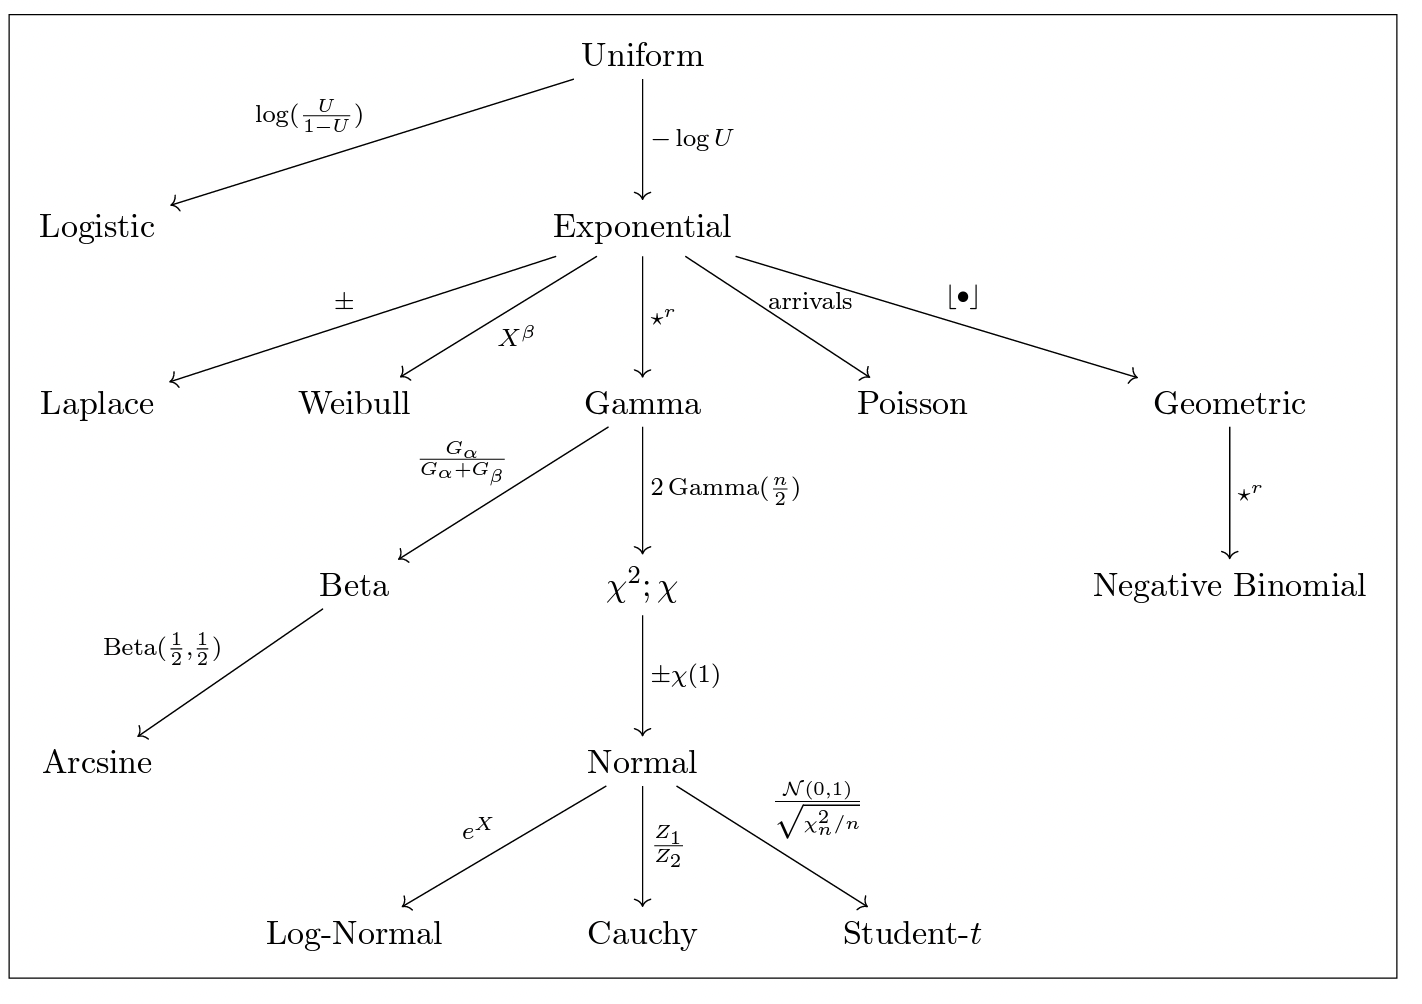
\includegraphics{./assets/img/derivation.png}

\hypertarget{pencil-3.3.2}{%
\subsection*{✏️ Pencil 3.3.2}\label{pencil-3.3.2}}
\addcontentsline{toc}{subsection}{✏️ Pencil 3.3.2}

Show that if \(U\sim Unif\), then \(1-U \sim Unif\). Also, show that
\(2U-1 \sim SU\) for \(S\) a random sign independent of \(U\) (so
\(2U-1\) is symmetric about 0, while \(U\) is symmetric about \(1/2\);
see Section 3.10 for more information.)

\begin{tcolorbox}[enhanced jigsaw, colback=white, left=2mm, leftrule=.75mm, breakable, bottomrule=.15mm, rightrule=.15mm, opacityback=0, arc=.35mm, colframe=quarto-callout-tip-color-frame, toprule=.15mm]
\begin{minipage}[t]{5.5mm}
\textcolor{quarto-callout-tip-color}{\faLightbulb}
\end{minipage}%
\begin{minipage}[t]{\textwidth - 5.5mm}

\textbf{Solution}\vspace{2mm}

Will release after section! :)

\end{minipage}%
\end{tcolorbox}

\hypertarget{pencil-3.4.12}{%
\subsection*{✏️ Pencil 3.4.12}\label{pencil-3.4.12}}
\addcontentsline{toc}{subsection}{✏️ Pencil 3.4.12}

Let \(Y_1\) and \(Y_2\) be r.v.s (possibly deifnied on different
\(\Omega\)'s) with CDFs \(F_1\) and \(F_2\) respectively. A commonly
used partial order on distributions (and thus on r.v.s),
\emph{stochastic domination} is defined by the relation
\(Y_1 \preceq Y_2\) iff \(F_1(y) \geq F_2(y)\) for all
\(y \in \mathbb{R}\).

Find an example of \(Y_1\) and \(Y_2\) on the same space with
\(Y_1 \preceq Y_2\) but \(P(Y_1 > Y_2) \geq 0.95\)

\begin{tcolorbox}[enhanced jigsaw, colback=white, left=2mm, leftrule=.75mm, breakable, bottomrule=.15mm, rightrule=.15mm, opacityback=0, arc=.35mm, colframe=quarto-callout-tip-color-frame, toprule=.15mm]
\begin{minipage}[t]{5.5mm}
\textcolor{quarto-callout-tip-color}{\faLightbulb}
\end{minipage}%
\begin{minipage}[t]{\textwidth - 5.5mm}

\textbf{Solution}\vspace{2mm}

Will release after section! :)

\end{minipage}%
\end{tcolorbox}

\hypertarget{pencil-3.5.10}{%
\subsection*{✏️ Pencil 3.5.10}\label{pencil-3.5.10}}
\addcontentsline{toc}{subsection}{✏️ Pencil 3.5.10}

Let \(W_1 \sim Wei(\beta_1), W_2 \sim Wei(\beta_2)\). Show that
\((W_1|W_1 \geq 1) \preceq (W_2|W_2 \geq 1)\) iff
\(\beta_1 \leq \beta_2\).

\begin{tcolorbox}[enhanced jigsaw, colback=white, left=2mm, leftrule=.75mm, breakable, bottomrule=.15mm, rightrule=.15mm, opacityback=0, arc=.35mm, colframe=quarto-callout-tip-color-frame, toprule=.15mm]
\begin{minipage}[t]{5.5mm}
\textcolor{quarto-callout-tip-color}{\faLightbulb}
\end{minipage}%
\begin{minipage}[t]{\textwidth - 5.5mm}

\textbf{Solution}\vspace{2mm}

Will release after section! :)

\end{minipage}%
\end{tcolorbox}

\hypertarget{pencil-3.6.16}{%
\subsection*{✏️ Pencil 3.6.16}\label{pencil-3.6.16}}
\addcontentsline{toc}{subsection}{✏️ Pencil 3.6.16}

Let \(C \sim\) Cauchy and \(U \sim\) Unif. Show that
\[tan(2 \pi U) \sim C\]

\begin{tcolorbox}[enhanced jigsaw, colback=white, left=2mm, leftrule=.75mm, breakable, bottomrule=.15mm, rightrule=.15mm, opacityback=0, arc=.35mm, colframe=quarto-callout-tip-color-frame, toprule=.15mm]
\begin{minipage}[t]{5.5mm}
\textcolor{quarto-callout-tip-color}{\faLightbulb}
\end{minipage}%
\begin{minipage}[t]{\textwidth - 5.5mm}

\textbf{Solution}\vspace{2mm}

Will release after section! :)

\end{minipage}%
\end{tcolorbox}

\hypertarget{pencil-3.7.18}{%
\subsection*{✏️ Pencil 3.7.18}\label{pencil-3.7.18}}
\addcontentsline{toc}{subsection}{✏️ Pencil 3.7.18}

Show that if \(C\sim\) Cauchy, \(S\) is a random sign, and \(B\sim\)
Beta(1/2, 1/2), then
\[C+\frac{1}{C} \sim 2S\sqrt{1+C^2}\sim \frac{2S}{\sqrt{B}}\]

\begin{tcolorbox}[enhanced jigsaw, colback=white, left=2mm, leftrule=.75mm, breakable, bottomrule=.15mm, rightrule=.15mm, opacityback=0, arc=.35mm, colframe=quarto-callout-tip-color-frame, toprule=.15mm]
\begin{minipage}[t]{5.5mm}
\textcolor{quarto-callout-tip-color}{\faLightbulb}
\end{minipage}%
\begin{minipage}[t]{\textwidth - 5.5mm}

\textbf{Solution}\vspace{2mm}

Will release after section! :)

\end{minipage}%
\end{tcolorbox}

\hypertarget{pencil-3.9.5}{%
\subsection*{✏️ Pencil 3.9.5}\label{pencil-3.9.5}}
\addcontentsline{toc}{subsection}{✏️ Pencil 3.9.5}

Show that NBin\((r,p)\) PMF is \(P(X=x)=\) \(r+x-1 \choose x\)
\(p^r q^x\), where \(q\equiv 1-p\).

\begin{tcolorbox}[enhanced jigsaw, colback=white, left=2mm, leftrule=.75mm, breakable, bottomrule=.15mm, rightrule=.15mm, opacityback=0, arc=.35mm, colframe=quarto-callout-tip-color-frame, toprule=.15mm]
\begin{minipage}[t]{5.5mm}
\textcolor{quarto-callout-tip-color}{\faLightbulb}
\end{minipage}%
\begin{minipage}[t]{\textwidth - 5.5mm}

\textbf{Solution}\vspace{2mm}

Will release after section! :)

\end{minipage}%
\end{tcolorbox}

\hypertarget{pencil-3.11.2}{%
\subsection*{✏️ Pencil 3.11.2}\label{pencil-3.11.2}}
\addcontentsline{toc}{subsection}{✏️ Pencil 3.11.2}

Suppose that \(Y_1, \cdots, Y_n \sim Expo\) are i.i.d. Show that the
minimum is also Exponentially distributed, with \(n\) times the rate:
\(Y_{(1)} \sim \frac{1}{n} Expo\) (the rate parameter is defined to be
reciprocal of the scale parameter)

\begin{tcolorbox}[enhanced jigsaw, colback=white, left=2mm, leftrule=.75mm, breakable, bottomrule=.15mm, rightrule=.15mm, opacityback=0, arc=.35mm, colframe=quarto-callout-tip-color-frame, toprule=.15mm]
\begin{minipage}[t]{5.5mm}
\textcolor{quarto-callout-tip-color}{\faLightbulb}
\end{minipage}%
\begin{minipage}[t]{\textwidth - 5.5mm}

\textbf{Solution}\vspace{2mm}

Will release after section! :)

\end{minipage}%
\end{tcolorbox}

\hypertarget{poisson-process}{%
\section*{Poisson Process}\label{poisson-process}}
\addcontentsline{toc}{section}{Poisson Process}

\markright{Poisson Process}

From Stat 110 textbook on pg 559:

\leavevmode\vadjust pre{\hypertarget{def-poisson-process}{}}%
\begin{definition}[]\label{def-poisson-process}

A sequence of arrivals in continuous time is a \emph{Poisson process}
with rate \(\lambda\) if the following conditions hold:

\begin{enumerate}
\def\labelenumi{\arabic{enumi}.}
\item
  The number of arrivals in an interval length \(t\) is distributed
  Pois\((\lambda t)\)
\item
  The numbers of arrivals in disjoint time intervals are independent.
\end{enumerate}

\end{definition}

Recall that in STAT 110, we also learn how to generate 1D Poisson
Process, detailed in pg 560 of the textbook:

\leavevmode\vadjust pre{\hypertarget{thm-poisson-story}{}}%
\begin{theorem}[]\label{thm-poisson-story}

(Generative Story for 1D Poisson process) To generate \(n\) arrivals
from a Poisson process on \((0, \infty)\) with rate \(\lambda\):

\begin{enumerate}
\def\labelenumi{\arabic{enumi}.}
\item
  Generate \(n\) i.i.d. Expo\((\lambda)\) r.v.s \(X_1, \cdots, X_n\)
\item
  For \(j=1, \cdots, n\), set \(T_j = X_1 + \cdots+X_j\)
\end{enumerate}

Then we can take \(T_1, \cdots, T_n\) to be the arrival times.

\emph{Ref: Story 13.1.2 in STAT 110 textbook}

\end{theorem}

Also note that on Theorem 13.2.1 in STAT 110 textbook:

\leavevmode\vadjust pre{\hypertarget{thm-conditional-counts}{}}%
\begin{theorem}[]\label{thm-conditional-counts}

(Conditional Counts) Let \((N(t):t>0)\) be a Poisson process with rate
\(\lambda\), and \(t_1<t_2\). The conditional distribution of \(N(t_1)\)
given \(N(t_2) = n\) is
\[N(t_1)|N(t_2)=n \sim Bin \left(n, \frac{t_1}{t_2}\right)\]

\end{theorem}

also note that Propositional 13.2.2 in STAT 110 textbook states that In
a Poisson process of rate \(\lambda\), conditional on \(N(t) =1\), the
first arrival time \(T_1\) has the Unif\((0,t)\) distribution.

Some other important concept about Poisson process from STAT 110
textbook include:

\leavevmode\vadjust pre{\hypertarget{thm-conditional-time}{}}%
\begin{theorem}[]\label{thm-conditional-time}

(Conditional times) In a process process of rate\(\lambda\), conditional
on \(N(t)=n\), the joint distribution of the arrival times
\(T_1, \cdots, T_n\) is the same as the joint distribution of the order
statistics of \(n\) i.i.d Unif\((0,t)\) r.v.s.

Also note that we know that the order statistics of Unif(0,1) r.v..s are
Betas, so the conditional distributions of the \(T_j\) are \emph{scaled}
Betas. To get Beta Distribution, we can just divide the \(T_j\) by \(t\)
so that their support is \((0,1)\):
\[t^{-1}T_j | N(t) = n \sim Beta(j, n-j+1)\]

\end{theorem}

\leavevmode\vadjust pre{\hypertarget{thm-poisson-story}{}}%
\begin{theorem}[]\label{thm-poisson-story}

(Generative Story for Poisson process) To generate \(n\) arrivals from a
Poisson process on \((0, t]\) with rate \(\lambda\):

\begin{enumerate}
\def\labelenumi{\arabic{enumi}.}
\item
  Generate the total number of events in the interval,
  \(N(t) \sim Pois(\lambda t)\)
\item
  Given \(N(t) = n\), generate \(n\) i.i.d Unif\((0,t)\) r.v.s
  \(U_1, \cdots, U_n\)
\item
  For \(j=1, \cdots, n\), set \(T_j = U_{(j)}\)
\end{enumerate}

\emph{Ref: Story 13.2.4 in STAT 110 textbook}

\end{theorem}

\leavevmode\vadjust pre{\hypertarget{thm-superposition}{}}%
\begin{theorem}[]\label{thm-superposition}

(Superposition). Let \((N_1(t): t>0)\) and \((N_2(t): t>0)\) be
independent Poisson process with rates \(\lambda_1\) and \(\lambda_2\)
respectively. Then the combined process \(N(t) = N_1(t) + N_2(t)\) is a
Poisson process with rate \(\lambda_1+\lambda_2\).

\end{theorem}

\leavevmode\vadjust pre{\hypertarget{thm-poisson-story-superposition}{}}%
\begin{theorem}[]\label{thm-poisson-story-superposition}

(Generative Story for superposition) To generate the superposition of
two independent Poisson processes, \((N_1(t): t>0)\) with
rate\(\lambda_1\), and \((N_2(t): t>0)\) with rate \(\lambda_2\):

\begin{enumerate}
\def\labelenumi{\arabic{enumi}.}
\item
  Generate arrivals from the Poisson process \((N_1(t): t>0)\)
\item
  Generate arrivals from the Poisson process \((N_2(t): t>0)\)
\item
  Superpose the results of steps 1 and 2.
\end{enumerate}

\emph{Ref: Story 13.2.7 in STAT 110 textbook}

\end{theorem}

There is also another generative story for superposition, as highlighted
below:

\leavevmode\vadjust pre{\hypertarget{thm-poisson-story-superposition-2}{}}%
\begin{theorem}[]\label{thm-poisson-story-superposition-2}

(Generative Story for superposition, take 2) To generate the
superposition of two independent Poisson processes, with
rate\(\lambda_1\) and \(\lambda_2\):

\begin{enumerate}
\def\labelenumi{\arabic{enumi}.}
\item
  Generate i.i.d Expo\((\lambda_1 +\lambda_2)\) r.v.s
  \(X_1, X_2,\cdots\) and let the \(j\)th arrival at time
  \(T_j =X_1+\cdots+X_j\)
\item
  Generate i.i.d r.v.s.
  \(I_1, I_2, \cdots Bern(\lambda_1/(\lambda_1+\lambda_2))\),
  independent of \(X_1, X_2, \cdots\). Let the \(j\)th arrival be type-1
  if \(I_j=1\), and type-2 otherwise.
\end{enumerate}

\emph{Ref: Story 13.2.9 in STAT 110 textbook}

\end{theorem}

Following up from the superposition definition and generative story
above, the two most important theorem arive from this are

\leavevmode\vadjust pre{\hypertarget{thm-superposition-discrete}{}}%
\begin{theorem}[]\label{thm-superposition-discrete}

(Projection of superposition into discrete time) Consider the
superposition \((N(t);t>0)\) of two independent Poisson processes with
rate \(\lambda_1\) and \(\lambda_2\). For \(j=1,2,\cdots\), let \(I_j\)
be the indicator of the \(j\)th event being from the Poisson process
with rate \(\lambda_1\). Then the \(I_j\) are i.i.d
Bern\((\lambda_1/(\lambda_1+\lambda_2))\)

\emph{Ref: Thm 13.2.11 in STAT 110 textbook}

\end{theorem}

Using the result above, we can orive wutg a story that a Gamma mixture
of Poissons is Negative Binomial:

\leavevmode\vadjust pre{\hypertarget{thm-mixture-poisson}{}}%
\begin{theorem}[]\label{thm-mixture-poisson}

(Exponential mixture of Poissons is Geometric). Suppose that
\(X \sim Expo(\lambda)\), and \(Y|X=x \sim Pois(\lambda)\). Then
\(Y\sim Geom(\lambda/(\lambda+1))\)

\emph{Ref: Thm 13.2.12 in STAT 110 textbook}

\end{theorem}

\leavevmode\vadjust pre{\hypertarget{thm-mixture-poisson-negative-binomial}{}}%
\begin{theorem}[]\label{thm-mixture-poisson-negative-binomial}

(Gamma mixture of Poissons is Negative Binomial). Suppose that
\(X \sim Gamma(r, \lambda)\), and \(Y|X=x \sim Pois(x)\). Then
\(Y\sim Nbin(r, \lambda/(\lambda+1))\)

\emph{Ref: Thm 13.2.12 in STAT 110 textbook}

\end{theorem}

\hypertarget{section-discussion-questions}{%
\section*{Section Discussion
Questions}\label{section-discussion-questions}}
\addcontentsline{toc}{section}{Section Discussion Questions}

\markright{Section Discussion Questions}

\hypertarget{section-problem-1-1}{%
\subsection*{✏️ Section Problem 1}\label{section-problem-1-1}}
\addcontentsline{toc}{subsection}{✏️ Section Problem 1}

Let \(A, B, C\) be i.i.d. Uniform\((0,1)\), which are coefficients of
the following ``random'\,' quadratic equation: \[
A x^2 + 2B x + C = 0.
\] What is the probability that the above equation has real root?

\begin{tcolorbox}[enhanced jigsaw, colback=white, left=2mm, leftrule=.75mm, breakable, bottomrule=.15mm, rightrule=.15mm, opacityback=0, arc=.35mm, colframe=quarto-callout-tip-color-frame, toprule=.15mm]
\begin{minipage}[t]{5.5mm}
\textcolor{quarto-callout-tip-color}{\faLightbulb}
\end{minipage}%
\begin{minipage}[t]{\textwidth - 5.5mm}

\textbf{Solution}\vspace{2mm}

Will release after section! :)

\end{minipage}%
\end{tcolorbox}

\hypertarget{section-problem-2-1}{%
\subsection*{✏️ Section Problem 2}\label{section-problem-2-1}}
\addcontentsline{toc}{subsection}{✏️ Section Problem 2}

Assume that \(U_1, \cdots, U_n \overset{i.i.d}{\sim}\) Unif,
\(Z_1, \cdots, Z_{2n} \overset{i.i.d}{\sim} \mathcal{N}(0,1)\), and the
\(U\)'s and \(Z\)'s are independent. Define \[
X = \frac{Z_1^2 + \cdots + Z_m^2}{ Z_1^2 + \cdots + Z_{2n}^2},
\] where \(m< 2n\). Find the distribution of
\(Y = (U_1 U_2 \cdots U_n)^{-X}\).

\begin{tcolorbox}[enhanced jigsaw, colback=white, left=2mm, leftrule=.75mm, breakable, bottomrule=.15mm, rightrule=.15mm, opacityback=0, arc=.35mm, colframe=quarto-callout-tip-color-frame, toprule=.15mm]
\begin{minipage}[t]{5.5mm}
\textcolor{quarto-callout-tip-color}{\faLightbulb}
\end{minipage}%
\begin{minipage}[t]{\textwidth - 5.5mm}

\textbf{Solution}\vspace{2mm}

Will release after section! :)

\end{minipage}%
\end{tcolorbox}

\hypertarget{section-problem-3-1}{%
\subsection*{✏️ Section Problem 3}\label{section-problem-3-1}}
\addcontentsline{toc}{subsection}{✏️ Section Problem 3}

Let \(Z_1, Z_2 \overset{i.i.d}{\sim} \mathcal{N}(0,1)\). Furthermore,
let \(X_1,X_2 \overset{i.i.d}{\sim} \chi_1^2\). Show that \[
Z_1Z_2\sim \frac{1}{2} (X_1 - X_2).
\]

\begin{tcolorbox}[enhanced jigsaw, colback=white, left=2mm, leftrule=.75mm, breakable, bottomrule=.15mm, rightrule=.15mm, opacityback=0, arc=.35mm, colframe=quarto-callout-tip-color-frame, toprule=.15mm]
\begin{minipage}[t]{5.5mm}
\textcolor{quarto-callout-tip-color}{\faLightbulb}
\end{minipage}%
\begin{minipage}[t]{\textwidth - 5.5mm}

\textbf{Solution}\vspace{2mm}

Will release after section! :)

\end{minipage}%
\end{tcolorbox}

\hypertarget{section-problem-4-1}{%
\subsection*{✏️ Section Problem 4}\label{section-problem-4-1}}
\addcontentsline{toc}{subsection}{✏️ Section Problem 4}

\begin{enumerate}
\def\labelenumi{(\alph{enumi})}
\item
  Let \(X_1, X_2 \overset{i.i.d}{\sim} Expo\). Show that
  \(X_1 - X_2 \sim \operatorname{Laplace}\).
\item
  Let \(Z_1,Z_2,Z_3,Z_4 \overset{i.i.d}{\sim} \mathcal{N}(0,1)\), and
  \(L \sim\) Laplace. Show that \[
  Z_1 Z_2 - Z_3 Z_4 \sim L.
  \]
\end{enumerate}

\begin{tcolorbox}[enhanced jigsaw, colback=white, left=2mm, leftrule=.75mm, breakable, bottomrule=.15mm, rightrule=.15mm, opacityback=0, arc=.35mm, colframe=quarto-callout-tip-color-frame, toprule=.15mm]
\begin{minipage}[t]{5.5mm}
\textcolor{quarto-callout-tip-color}{\faLightbulb}
\end{minipage}%
\begin{minipage}[t]{\textwidth - 5.5mm}

\textbf{Solution}\vspace{2mm}

Will release after section! :)

\end{minipage}%
\end{tcolorbox}

\hypertarget{section-problem-5-1}{%
\subsection*{✏️ Section Problem 5}\label{section-problem-5-1}}
\addcontentsline{toc}{subsection}{✏️ Section Problem 5}

Let \(Y\) have a Cauchy distribution centered at \(\theta\), i.e.~the
density of \(Y\) is
\[f(y|\theta) = \frac{1}{\pi} \frac{1}{1+(y-\theta)^2} ,\hspace{0.2cm} y \in \mathbb{R} \]
Suppose that \(\theta\) has a Cauchy distribution (centered at \(0\)).
Find the marginal distribution of \(Y\).

\begin{tcolorbox}[enhanced jigsaw, colback=white, left=2mm, leftrule=.75mm, breakable, bottomrule=.15mm, rightrule=.15mm, opacityback=0, arc=.35mm, colframe=quarto-callout-tip-color-frame, toprule=.15mm]
\begin{minipage}[t]{5.5mm}
\textcolor{quarto-callout-tip-color}{\faLightbulb}
\end{minipage}%
\begin{minipage}[t]{\textwidth - 5.5mm}

\textbf{Solution}\vspace{2mm}

Will release after section! :)

\end{minipage}%
\end{tcolorbox}

\hypertarget{section-problem-6-1}{%
\subsection*{✏️ Section Problem 6}\label{section-problem-6-1}}
\addcontentsline{toc}{subsection}{✏️ Section Problem 6}

The people of Lineland live on the unit interval \([0,1]\). They love
coffee. Currently, they have 2 Starbucks stores, at the points 0 and 1.
Starbucks decides to open new stores in Lineland, according to a Poisson
process of rate \(\lambda\) on the interval \([0,1]\). Let \(N\) be the
number of new Starbucks stores in Lineland (i.e., not including the
existing stores at the points 0 and 1 ). Let \(W\) be the furthest
distance that a Lineland citizen could ever have to walk to get to the
nearest Starbucks, after the new stores have opened. Find
\(E(W \mid N=n)\), where \(n\) is a positive integer. Simplify fully,
expressing your answer in terms of a harmonic number \(H_m\) for some
\(m\), where \[
H_m=\sum_{k=1}^m \frac{1}{k} .
\]

\begin{tcolorbox}[enhanced jigsaw, colback=white, left=2mm, leftrule=.75mm, breakable, bottomrule=.15mm, rightrule=.15mm, opacityback=0, arc=.35mm, colframe=quarto-callout-tip-color-frame, toprule=.15mm]
\begin{minipage}[t]{5.5mm}
\textcolor{quarto-callout-tip-color}{\faLightbulb}
\end{minipage}%
\begin{minipage}[t]{\textwidth - 5.5mm}

\textbf{Solution}\vspace{2mm}

Will release after section! :)

\end{minipage}%
\end{tcolorbox}

\hypertarget{section-problem-7}{%
\subsection*{✏️ Section Problem 7}\label{section-problem-7}}
\addcontentsline{toc}{subsection}{✏️ Section Problem 7}

Consider the following simple model for the growth of a population of
bacteria. Any individual bacterium splits into two bacteria at some
random time, independently. It takes an Exponential amount of time for
any specific bacterium to split (measured from the time of birth of that
bacterium, and choosing the units in which time is measured so that the
Expo has mean 1). So each individual bacterium has its own Expo waiting
time until it splits, and these Expo r.v.s are i.i.d.

At time 0 , there is one bacterium. Let \(T_n\) be the time (on a
timeline) of the \(n\)th splitting occurrence. So \(T_1<T_2<\ldots\),
with \(T_1\) the time at which the bacterium that was present at time 0
splits, \(T_2\) the time of the next splitting occurrence, etc.

\begin{enumerate}
\def\labelenumi{(\alph{enumi})}
\item
  Find the CDF of \(T_n\).
\item
  Find the distribution of the number of bacteria present at time \(t\),
  for any \(t>0\).
\end{enumerate}

\begin{tcolorbox}[enhanced jigsaw, colback=white, left=2mm, leftrule=.75mm, breakable, bottomrule=.15mm, rightrule=.15mm, opacityback=0, arc=.35mm, colframe=quarto-callout-tip-color-frame, toprule=.15mm]
\begin{minipage}[t]{5.5mm}
\textcolor{quarto-callout-tip-color}{\faLightbulb}
\end{minipage}%
\begin{minipage}[t]{\textwidth - 5.5mm}

\textbf{Solution}\vspace{2mm}

Will release after section! :)

\end{minipage}%
\end{tcolorbox}

\hypertarget{section-problem-8}{%
\subsection*{✏️ Section Problem 8}\label{section-problem-8}}
\addcontentsline{toc}{subsection}{✏️ Section Problem 8}

In a certain town, each married couple has a Poisson \((\lambda)\)
number of children, with \(\lambda\) unknown. An anthropologist picks a
sample of couples and observes \(Y_1, \ldots, Y_n\), where \(Y_j\) is
the number of children of the \(j\) th couple and it is assumed that
\(Y_j \sim \operatorname{Pois}(\lambda)\) independently. The
anthropologist wishes to estimate the probability of a couple being
childless, i.e., \(p_0 \equiv P\left(Y_j=0\right)\). Let \(\bar{Y}\) be
the sample mean of \(Y_1, \ldots, Y_n\).

\begin{enumerate}
\def\labelenumi{(\alph{enumi})}
\item
  Find \(E\left(Y_1 \mid \bar{Y}\right)\) and the conditional
  distribution of \(Y_1\) given \(\bar{Y}\).
\item
  The anthropologist proposes estimating \(p_0\) using the proportion of
  couples that are childless, i.e., the number of childless couples
  divided by \(n\). Call this estimator \(T\). It will be shown later in
  Stat \(210 / 211\) that a better estimator can be obtained by
  conditioning on \(\bar{Y}\). Find a simple expression for
  \(E(T \mid \bar{Y})\) (this new estimator should be computable without
  knowing \(\lambda\) ).
\end{enumerate}

\begin{tcolorbox}[enhanced jigsaw, colback=white, left=2mm, leftrule=.75mm, breakable, bottomrule=.15mm, rightrule=.15mm, opacityback=0, arc=.35mm, colframe=quarto-callout-tip-color-frame, toprule=.15mm]
\begin{minipage}[t]{5.5mm}
\textcolor{quarto-callout-tip-color}{\faLightbulb}
\end{minipage}%
\begin{minipage}[t]{\textwidth - 5.5mm}

\textbf{Solution}\vspace{2mm}

Will release after section! :)

\end{minipage}%
\end{tcolorbox}

\hypertarget{next-week-1}{%
\section*{Next Week}\label{next-week-1}}
\addcontentsline{toc}{section}{Next Week}

\markright{Next Week}

Next week, we will discuss:

\begin{itemize}
\tightlist
\item
  On Order Statistics
\item
  Meaning on Mean
\end{itemize}

Feel free to upload the pencil problem you wish to be discussed next
week \href{https://forms.gle/RBmMNYJp4u3qD5W79}{here}.

Note that a verified email address is needed in the GForm so we don't
get scammy input! :)

\(\,\)

\bookmarksetup{startatroot}

\hypertarget{meme-quotes}{%
\chapter*{Meme \& Quotes}\label{meme-quotes}}
\addcontentsline{toc}{chapter}{Meme \& Quotes}

\markboth{Meme \& Quotes}{Meme \& Quotes}

\hypertarget{quotes}{%
\section*{Quotes}\label{quotes}}
\addcontentsline{toc}{section}{Quotes}

\markright{Quotes}

\begin{quote}
How will our participation grade be measured? \emph{Joe}: Using measure
theory.
\end{quote}

\begin{quote}
Measure theory is just about measuring things - Jun Liu, Spring 2023
\end{quote}

\begin{quote}
What I don't like about measure theory is that you have to say ``almost
everywhere'' almost everywhere. - Kurt Friedrichs
\end{quote}

\hypertarget{meme}{%
\section*{Meme}\label{meme}}
\addcontentsline{toc}{section}{Meme}

\markright{Meme}


\includegraphics[width=5.20833in,height=3.125in]{./assets/img/meme/meme1.png}

\includegraphics[width=5.20833in,height=3.125in]{./assets/img/meme/meme3.jpeg}

\includegraphics[width=5.20833in,height=7.29167in]{./assets/img/meme/meme2.webp}

\hypertarget{upload-your-meme-quotes}{%
\section*{Upload your meme / quotes}\label{upload-your-meme-quotes}}
\addcontentsline{toc}{section}{Upload your meme / quotes}

\markright{Upload your meme / quotes}

If you would like to contribute to this meme + quotes page, please
upload it at this \href{https://forms.gle/RBmMNYJp4u3qD5W79}{form}

Note that a verified email address is needed in the GForm so we don't
get scammy input! :)

\(\,\)



\end{document}
